% MANUAL DE ATUALIZAÇÃO DO PCC, página 20/21
%Passo 5 - Realizados os passos anteriores inicia-se a elaboração do desenho/esboço
%geral do currículo. Sugere-se ao grupo de trabalho, com o intuído de facilitar a organização do
%currículo, a utilização de um desenho gráfico do currículo (esboço conceitual das inter-relações),
%com uso as ferramentas gráficas, tabelas, fluxogramas, design conceitual entre outros, para
%melhor visualização das inter-relações entre as experiências de ensino-aprendizagem, os
%objetivos de aprendizagem e a avaliação da aprendizagem, tríade responsável pelo
%desenvolvimento das competências.
%O currículo é o grande norteador do processo educacional. Ele contempla todas as
%estratégias de aprendizagem, atividades de ensino/pesquisa/extensão, processos avaliativos,
%metodologias e demais aspectos necessários ao desenvolvimento dos estudantes. O currículo
%deve apresentar, claramente, o caminho formativo que o estudante percorrerá no curso. Assim,
%nesse ponto do trabalho, a equipe deve:
%►
%sugerir/desenvolver/pensar/criar/adaptar estratégias metodológicas de ensino-
%aprendizagem capazes de potencializar/desenvolver/aflorar as competências identificadas no
%passo 3.
%►
%representar, graficamente, a matriz de desenvolvimento das competências. Aqui
%sugere-se a substituição da matriz curricular utilizada nos PPC atuais do IFCE por matrizes que
%utilizam estratégias pedagógicas inovadoras e atualizadas com as questões contemporâneas.
%Para efeito de exemplo pode-se destacar o modelo de matriz circular.
%►
%sugerir/desenvolver/pensar/criar/adaptar estratégias de avaliação para identificar
%os níveis de desenvolvimento das competências nos estudantes. Uma dica para criar
%situações/momentos/atividades de avaliação para auxiliar a elaboração do curriculo é pensar
%nos indicadores que serão avaliados em cada momento de desenvolvimento da competência.
%20MINUTA - Manual de Normalização de Projetos Pedagógicos dos cursos de engenharia do IFCE
%Esses indicadores, também chamados de rubricas, são elementos que orientam o processo de
%avaliação como um todo, ao mesmo tempo que indicam, ao estudante, o que será avaliado
%naquele momento de aprendizagem, ajudam ao docente a elaborar uma avaliação bem
%direcionada. Importante deixar claro que essa sugestão auxilia o processo de elaboração do
%desenho do currículo e não se configura como elemento essencial no texto. A rubrica pode ser
%pensada por atividades individuais dentro das disciplinas por exemplo ou de forma sistêmica,
%abrangendo todas as atividades do curso. O importante é valorizar o esforço do estudante.
%O uso de rubricas pode auxiliar o professor na elaboração de conteúdos e na conexão
%com os demais conteúdos e atividades do currículo
%



\section{ESTRUTURA CURRICULAR}
A estrutura curricular do \NOMECURSO é dividida nos seguintes itens: 

\begin{itemize}
	\item Organização Curricular 
	\item Matriz curricular 
	\item Fluxograma
	\item Estágio
	\item Atividades complementares 
	\item Projeto de final de curso (PFC). 
\end{itemize}



\subsection{Organização Curricular}
Na organização curricular do \NOMECURSO foram considerados princípios que orientam a formação profissional e atendem ao perfil do egresso, conforme a seguir:

\begin{itemize}
	\item \textbf{Formação Básica Sólida}: assegurada por um conjunto de disciplinas obrigatórias fundamentais à área do \NOMECURSO, garantindo a base científica e tecnológica necessária ao desenvolvimento das competências profissionais;
	\item \textbf{Flexibilidade Curricular}: possibilita ao estudante complementar sua formação com disciplinas optativas e atividades acadêmicas diversas (estágio, iniciação científica, projetos, entre outras), de acordo com seus interesses técnico-profissionais;
	\item \textbf{Atualização Permanente}: a estrutura curricular facilita a incorporação de novas tecnologias, metodologias e conceitos, especialmente por meio de componentes optativos e atividades formativas;
	\item \textbf{Qualidade da Formação}: além das atividades teóricas, o currículo prevê vivências práticas e integradoras, incluindo estágios, projetos de conclusão de curso, atividades de iniciação científica e disciplinas de caráter articulador, promovendo o amadurecimento técnico e crítico do estudante;
	\item \textbf{Interdisciplinaridade}: os conteúdos do núcleo de formação básica articulam-se entre si e com os componentes específicos, favorecendo a integração de saberes, inclusive com possibilidade de cursá-los em outros cursos do IFCE.
\end{itemize}

De modo geral, a proposta curricular organiza-se em um conjunto de disciplinas obrigatórias e outro de disciplinas optativas, conforme cargas horárias definidas na Tab.~\ref{tab4}, resultante da atuação contínua e integrada do Núcleo Docente Estruturante (NDE) e do Colegiado do Curso.

%\clearpage
%\thispagestyle{empty}
\begin{longtable}{|p{0.3cm}|p{7.1cm}|p{2.7cm}|p{1.8cm}|p{1.0cm}|}
	\caption{Distribuição da Carga Horária do Curso}\label{tab4}
	
	\vspace{-0.25cm} \\
	\hline 
	\cellcolor{\cinza} & \cellcolor{\cinza}Atividades & \cellcolor{\cinza}máximo de horas-aula semanais & \cellcolor{\cinza}horas-aula totais & \cellcolor{\cinza}[\%] \\ 
	\hline
	1 &  Disciplinas Obrigatórias  &  \CHTOTALDOBSE  &  \CHTOTALDOB & \CHTOTALDOBPE \\ \hline
	2 &  Disciplinas Optativas Obrigatórias  &  \CHOPTMINSE  &  \CHOPTMIN & \CHOPTMINPE \\ \hline
	3 &  Estágio  &  \CHESTAGIOSE  &  \CHESTAGIO & \CHESTAGIOPE \\ \hline
	4 &  Total Obrigatório  &  \CHTOTALOBSE  &  \CHTOTALOB & \CHTOTALOBPE \\ \hline

	5 &  Atividades Complementares Não Obrigatórias &  \CHCOMPSE  &  \CHCOMP & \CHCOMPPE \\ \hline

\end{longtable}

A Tab. \ref{tab5} apresenta o conjunto de disciplinas de conteúdo básico que compõem a proposta curricular. As Tabs. \ref{tab6} e \ref{tab7} apresentam, respectivamente, as disciplinas de conteúdo profissionalizante e de conteúdo específico (optativas). As denominações “conteúdo básico”, “conteúdo profissionalizante” e “conteúdo específico” seguem a classificação estabelecida pela \citeonline{cne19}.

As disciplinas de conteúdo básico possuem caráter integrador no âmbito do campus, por serem comuns aos cursos de engenharia e promoverem, desde os semestres iniciais, a interação acadêmica entre os estudantes das diferentes áreas.

Destaca-se, ainda, que a definição das disciplinas que integram a matriz curricular, bem como suas respectivas cargas horárias, resulta da atuação contínua e articulada entre o Núcleo Docente Estruturante (NDE) e o Colegiado do Curso, assegurando coerência formativa e alinhamento ao perfil do egresso.


\begin{destacar}
	

\begin{longtable}{|p{0.8cm}|p{7.5cm}|p{2.0cm}|} 
	\caption{Disciplinas de conteúdo básico}\label{tab5} 
	\vspace{-0.25cm}
	\\ \hline 
	\cellcolor{\cinza} & \cellcolor{\cinza}Disciplinas & \cellcolor{\cinza}horas-aula semanais  \\ 
	\hline
	1 &  Introdução à Engenharia  &  2 \\ \hline
	2 &  Cálculo I  &  4 \\ \hline
	3 &  Cálculo II  &  4 \\ \hline
	4 &  Cálculo III  &  4 \\ \hline
	5 &  Física I  &  4 \\ \hline
	6 &  Física II  &  4 \\ \hline
	7 &  Física III  &  4 \\ \hline
	8 &  Álgebra Linear  &  4 \\ \hline
	9 &  Química Geral  &  4 \\ \hline
	10 &  Inglês Técnico  &  2 \\ \hline
	11 &  Probabilidade e Estatística  &  4 \\ \hline
	12 &  Desenho Técnico  &  4 \\ \hline
	13 &  Desenho Auxiliado por Computador  &  4 \\ \hline
	14 &  Lógica de Programação  &  4 \\ \hline
	15 &  Linguagem de Programação  &  4 \\ \hline
	16 &  HST  &  2 \\ \hline
	17 &  Metodologia Científica e Tecnológica  &  2 \\ \hline
	18 &  Ética e Cidadania  &  2 \\ \hline
	19 &  Projetos Sociais  &  2 \\ \hline
	&  Total / (\% em relação à carga total obrigatória)  &  \CHBASICACR(\CHBASICAPEMIN) \\ \hline
\end{longtable}

\begin{longtable}{|p{0.8cm}|p{7.5cm}|p{2.0cm}|}
	\caption{Disciplinas de conteúdo profissionalizante}\label{tab6} 
	\vspace{-0.25cm}
	\\ \hline 
	\cellcolor{\cinza} & \cellcolor{\cinza}Disciplinas & \cellcolor{\cinza}horas-aula semanais  \\ 
	\hline
	1 &  Metrologia  &  4 \\ \hline
	2 &  Eletrônica I  &  4 \\ \hline
	3 &  Materiais I  &  4 \\ \hline
	4 &  Circuitos Elétricos I  &  4 \\ \hline
	5 &  Métodos Numéricos  &  4 \\ \hline
	6 &  Eletrônica II  &  4 \\ \hline
	7 &  Circuitos Elétricos II  &  4 \\ \hline
	8 &  Instrumentação  &  4 \\ \hline
	9 &  Sistemas Lineares  &  4 \\ \hline
	10 &  Resistência dos Materiais I  &  4 \\ \hline
	11 &  Microcontroladores  &  4 \\ \hline
	12 &  Eletrônica III  &  4 \\ \hline
	13 &  Instalações Elétricas  &  4 \\ \hline
	14 &  Controle I  &  4 \\ \hline
	15 &  Processamento Digital de Sinais  &  4 \\ \hline
	16 &  Controladores Lógicos Programáveis  &  4 \\ \hline
	17 &  Máquinas Elétricas  &  4 \\ \hline
	18 &  Acionamentos Hidráulicos e Pneumáticos  &  4 \\ \hline
	19 &  Empreendedorismo  &  2 \\ \hline
	20 &  Controle II  &  4 \\ \hline
	21 &  Acionamento de Máquinas  &  4 \\ \hline
	22 &  Dispositivos Periféricos  &  4 \\ \hline
	23 &  Robótica I  &  4 \\ \hline
	24 &  Sistemas Digitais de Controle Distribuído  &  4 \\ \hline
	25 &  Manufatura Auxiliada por Computador  &  4 \\ \hline
	26 &  Gestão e Controle da Qualidade  &  4 \\ \hline
	27 &  Gestão da Manutenção Industrial &  4 \\ \hline
	28 &  PFC  &  4 \\ \hline
	29 &  Estágio Currícular  &  20 \\ \hline
	&  Total / (\% em relação à carga total obrigatória)  &  \CHPROFCR(\CHPROFPEMIN) \\ \hline
\end{longtable}

\begin{longtable}{|p{0.8cm}|p{7.5cm}|p{2.0cm}|}
	\caption{Disciplinas de conteúdo específico (optativas)}\label{tab7} 
	\vspace{-0.25cm}
	\\ \hline 
	\cellcolor{\cinza} & \cellcolor{\cinza}Disciplinas & \cellcolor{\cinza}horas-aula semanais  \\ 
	\hline
	1 &  Manufatura Integrada por Computador  &  4 \\ \hline
	2 &  Modelagem de Sistemas a Eventos Discretos  &  4 \\ \hline
	3 &  Processamento Digital de Imagens  &  4 \\ \hline
	4 &  Robótica II  &  4 \\ \hline
	5 &  Identificação de Sistemas  &  4 \\ \hline
	6 &  Sistemas Embarcados  &  4 \\ \hline
	7 &  Controle III  &  4 \\ \hline
	8 &  Equações Diferênciais Ordinárias  &  4 \\ \hline
	9 &  Inteligência Computacional Aplicada  &  4 \\ \hline
	10 &  Mecânica dos Fluidos  &  4 \\ \hline
	11 &  Libras  &  4 \\ \hline
	12 &  Educação Física  &  2 \\ \hline
	&  Total / (\% em relação à carga total obrigatória)  &  \CHOPTCR(\CHOPTPEMIN) \\ \hline
\end{longtable}

\begin{longtable}{|p{0.8cm}|p{7.5cm}|p{2.0cm}|}
	\caption{Disciplinas de conteúdo específico (optativas)}\label{tab7} 
	\vspace{-0.25cm}
	%\multicolumn{3}{c}{\textbf{Tabela 4. Disciplinas de conteúdo específico (optativas)}}\label{tab7} 
	\\ \hline 
	\cellcolor{\cinza} & \cellcolor{\cinza}Disciplinas & \cellcolor{\cinza}horas-aula semanais  \\ 
	\hline
	1 &  Corrosão e Proteção Anti-Corrosiva  &  4 \\ \hline
	2 &  Tribologia e Lubrificação  &  4 \\ \hline
	3 &  Transportadores Industriais  &  4 \\ \hline
	4 &  Gestão de Projetos  &  4 \\ \hline
	5 &  Projeto de Engenharia  &  4 \\ \hline
	6 &  Manufatura Integrada por Computador  &  4 \\ \hline
	7 &  Processamento Digital de Imagens  &  4 \\ \hline
	8 &  Equações Diferênciais Ordinárias  &  4 \\ \hline
	9 &  Inteligência Computacional Aplicada  &  4 \\ \hline
	10 &  Libras  &  4 \\ \hline
	11 &  Educação Física  &  2 \\ \hline
	&  Total / (\% em relação à carga total obrigatória)  &  \CHOPTCR(\CHOPTPEMIN) \\ \hline
\end{longtable}

\end{destacar}

Embora o \NOMECURSO adote organização anual, as disciplinas de conteúdo básico são ofertadas semestralmente no \textit{campus}, tanto no próprio curso quanto em outros cursos de engenharia. Essa política visa mitigar retenção e evasão, permitindo ao estudante que, em caso de reprovação, desistência ou trancamento, possa cursar novamente a disciplina no semestre imediatamente subsequente.


\subsection{Matriz Curricular}

A Matriz Curricular do \NOMECURSO do IFCE \textit{Campus} Maracanaú, apresentada na Tab.~\ref{MATRIZ}, contempla todas as disciplinas que compõem o curso. A organização curricular está distribuída em 10 (dez) semestres letivos, cada qual estruturado em 100 dias de atividades acadêmicas. Em cada semestre, são desenvolvidas Unidades Curriculares com objetivos e habilidades claramente definidos, assegurando que, ao final da formação, o egresso alcance o conjunto de competências requeridas para o exercício profissional.

A matriz contempla disciplinas de formação básica, profissionalizante e específica, garantindo sólida preparação teórica e prática. Ao longo do curso, o discente deverá cursar, no mínimo, duas disciplinas optativas de conteúdo específico, totalizando 160 horas. Considerando a política de flexibilização curricular, busca-se ofertar, em cada semestre, pelo menos uma disciplina optativa prevista na matriz, de modo a garantir a disponibilidade integral do conjunto de componentes opcionais. Ressalta-se que, para cursar tais disciplinas, devem ser observados os pré-requisitos estabelecidos.

O discente poderá solicitar aproveitamento de disciplinas específicas ou optativas cursadas em outros cursos de nível equivalente pertencentes ao Eixo Tecnológico da Indústria, conforme normas institucionais vigentes.

Em atendimento ao Decreto Federal nº 5.626, de 22 de dezembro de 2005, Capítulo II, Art. 3º, §2º, consta na matriz curricular a disciplina optativa de Língua Brasileira de Sinais – LIBRAS. O texto integral do Decreto encontra-se no ANEXO~\ref{anexoDecreto}.

As componentes curriculares do \NOMECURSO encontram-se detalhadas em seus respectivos Programas de Unidade Didática (PUD), que especificam pré-requisitos, carga horária (total, teórica e prática), créditos, período, relações interdisciplinares, ementa, objetivos, conteúdos, metodologias, critérios de avaliação, recursos e bibliografias básica e complementar. Os PUDs são revisados sempre que necessário, assegurando atualização e aderência às demandas acadêmicas e profissionais. A relação completa dos PUDs está apresentada no ANEXO~\ref{anexoPUD}.

A matrícula é requerida pelo estudante e efetivada por Unidades Curriculares, conforme prazos definidos no calendário acadêmico do Campus Maracanaú. O regime de matrícula segue as disposições das Seções I e II, Capítulo II, Título III, do Regulamento da Organização Didática (ROD), de junho de 2015 (ANEXO~\ref{anexoRODmatricula}). No primeiro semestre, a matrícula é integral e obrigatória em todas as disciplinas previstas; a partir do segundo semestre, o discente pode realizar a escolha de disciplinas. O tempo mínimo para integralização do curso é de 10 (dez) semestres letivos.

\begin{destacar}

 \begin{longtable}{|c|c|l|c|c|p{1.5cm}|}
 \caption{MATRIZ CURRICULAR ECA (5719)} \label{MATRIZ}
 
 \vspace{-0.25cm}
 %\multicolumn{6}{c}{\textbf{Tabela 5. MATRIZ CURRICULAR ECA (5719)}} \label{MATRIZ}
 
 \\ \hline 

 \cellcolor{\cinza}Sem & \cellcolor{\cinza}Cod & \cellcolor{\cinza}Disciplina & \cellcolor{\cinza}CH & \cellcolor{\cinza}CR & \cellcolor{\cinza}PR \\ 

 \hline 
\hline

S1&  \hyperref[PUD:ACE002]{04507.1} & Álgebra Linear & 80 & 4 &  \\ 

S1&  \hyperref[PUD:ACE003]{04507.2} & Cálculo 1 & 80 & 4 &  \\ 

S1&  \hyperref[PUD:ACE004]{04507.3} & Inglês Técnico & 40 & 2 &  \\ 

S1&  \hyperref[PUD:ACE005]{04507.4} & Química Geral & 80 & 4 &  \\ 

S1&  \hyperref[PUD:ACE017]{04507.5} & Introdução à Engenharia & 40 & 2 & \\ 

S1&  \hyperref[PUD:EME105]{04507.6} & Desenho Técnico & 80 & 4 & \\ 

& & & \fbox{\textbf{400}} & & \\ 
\hline

%S2&  \hyperref[PUD:ACE006]{04507.7} & Cálculo 2 & 80 &  \hyperref[PUD:ACE002]{04507.1}  \hyperref[PUD:ACE003]{04507.2}  \\ 
S2&  \hyperref[PUD:ACE006]{04507.7} & Cálculo 2 & 80 & 4 &  \hyperref[PUD:ACE003]{04507.2} \\ 

S2&  \hyperref[PUD:ACE008]{04507.8} & Física 1 & 80 & 4 &  \hyperref[PUD:ACE003]{04507.2} \\ 

S2&  \hyperref[PUD:ACE013]{04507.9} & Probabilidade e Estatística & 80 & 4 &  \hyperref[PUD:ACE003]{04507.2} \\ 

S2&  \hyperref[PUD:ECA208]{04507.10} & Lógica de Programação & 80 & 4 &  \\ 

S2&  \hyperref[PUD:EME106]{04507.11} & Desenho Auxiliado por Computador & 80 & 4 &  \hyperref[PUD:EME105]{04507.6}  \\ 

& & & \fbox{\textbf{400}} & & \\ 
\hline

S3&  \hyperref[PUD:ACE010]{04507.12} & Cálculo 3 & 80 & 4 &  \hyperref[PUD:ACE006]{04507.7} \\ 

S3&  \hyperref[PUD:ACE011]{04507.13} & Física 2 & 80 & 4 &  \hyperref[PUD:ACE008]{04507.8} \\ 

S3&  \hyperref[PUD:ECA209]{04507.14} & Linguagem de Programação & 80 & 4 &  \hyperref[PUD:ECA208]{04507.10} \\ 

S3&  \hyperref[PUD:ECA211]{04507.15} & Eletrônica I & 80 & 4 & \\ 

S3&  \hyperref[PUD:EME107]{04507.16} & Metrologia & 80 & 4 & \\ 

& & & \fbox{\textbf{400}} & & \\ 
\hline

S4&  \hyperref[PUD:ACE009]{04507.17} & HST & 40 & 2 & \\ 

S4&  \hyperref[PUD:ACE012]{04507.18} & Física 3 & 80 & 4 &  \hyperref[PUD:ACE011]{04507.13} \\ 

S4&  \hyperref[PUD:ACE014]{04507.19} & Metodologia Científica e Tecnológica & 40 & 2 &  \\ 

S4&  \hyperref[PUD:ECA210]{04507.20} & Circuitos Elétricos I & 80 & 4 &  \hyperref[PUD:ACE003]{04507.2} \\ 

S4&  \hyperref[PUD:ECA212]{04507.21} & Métodos Numéricos & 80 & 4 &  \hyperref[PUD:ECA209]{04507.14}  \\ 

S4&  \hyperref[PUD:EME108]{04507.22} & Materiais & 80 & 4 &  \hyperref[PUD:ACE005]{04507.4}  \\ 

& & & \fbox{\textbf{400}} & & \\ 
\hline

S5&  \hyperref[PUD:ECA214]{04507.23} & Eletrônica II & 80 & 4 &  \hyperref[PUD:ECA210]{04507.20} \\ 

S5&  \hyperref[PUD:ECA215]{04507.24} & Circuitos Elétricos II & 80 & 4 &  \hyperref[PUD:ECA210]{04507.20} \\ 

S5&  \hyperref[PUD:ECA219]{04507.25} & Instrumentação & 80 & 4 & \\ 

S5&  \hyperref[PUD:ECA220]{04507.26} & Sistemas Lineares & 80 & 4 &  \hyperref[PUD:ACE002]{04507.1} \\ 

S5&  \hyperref[PUD:EME109]{04507.27} & Resistência dos Materiais & 80 & 4 &  \hyperref[PUD:EME108]{04507.22}  \\ 

& & & \fbox{\textbf{400}} & &  \\ 
\hline

S6&  \hyperref[PUD:ECA213]{04507.28} & Microcontroladores & 80 & 4 &  \hyperref[PUD:ECA209]{04507.14}  \\ 

S6&  \hyperref[PUD:ECA216]{04507.29} & Eletrônica III & 80 & 4 &  \hyperref[PUD:ECA214]{04507.23} \\ 

S6&  \hyperref[PUD:ECA222]{04507.30} & Instalações Elétricas & 80 & 4 &  \hyperref[PUD:ECA210]{04507.20} \\ 

S6&  \hyperref[PUD:ECA233]{04507.31} & Controle I & 80 & 4 & \hyperref[PUD:ECA220]{04507.24} \\ 

& & & \fbox{\textbf{320}} & & \\ 
\hline

S7&  \hyperref[PUD:ACE007]{04507.33} & Ética e Cidadania & 40 & 2 & \\ 

S7&  \hyperref[PUD:ECA205]{04507.34} & Processamento Digital de Sinais & 80 & 4 &  \hyperref[PUD:ECA220]{04507.26}\\ 

S7&  \hyperref[PUD:ECA221]{04507.35} & Controladores Lógicos Programáveis & 80 & 4 & \hyperref[PUD:ECA213]{04507.28}\\ 

S7&  \hyperref[PUD:ECA223]{04507.36} & Máquinas Elétricas & 80 & 4 & \hyperref[PUD:ACE012]{04507.18} \\ 

S7&  \hyperref[PUD:ECA228]{04507.37} & Acionamentos Hidráulicos e Pneumáticos & 80 & 4 &  \hyperref[PUD:ECA214]{04507.30}  \\ 

& & & \fbox{\textbf{360}} & & \\ 
\hline

S8&  \hyperref[PUD:ACE015]{04507.38} & Empreendedorismo & 40 & 2 & \\ 

%S8&  \hyperref[PUD:ACE018]{04507.39} & Tópicos Especiais em Engenharia I & 80 &  \\ 

S8&  \hyperref[PUD:ECA202]{04507.40} & Controle II & 80 & 4 & \hyperref[PUD:ECA233]{04507.31} \\ 

S8&  \hyperref[PUD:ECA224]{04507.41} & Acionamento de Máquinas & 80 & 4 & \hyperref[PUD:ECA233]{04507.31} \\ 

S8&  \hyperref[PUD:ECA225]{04507.42} & Dispositivos Periféricos & 80 & 4 &  \hyperref[PUD:ECA213]{04507.28}  \\

& & & \fbox{\textbf{280}} & & \\ 
\hline

%S9&  \hyperref[PUD:ACE019]{04507.43} & Tópicos Especiais em Engenharia II & 80 &  \\ 

S9&  \hyperref[PUD:ECA226]{04507.44} & Robótica I & 80 & 4 &  \hyperref[PUD:ECA225]{04507.42}  \\ 

S9&  \hyperref[PUD:ECA227]{04507.45} & Sistemas Digitais de Controle Distribuído & 80 & 4 &  \\ 

S9&  \hyperref[PUD:EME123]{04507.46} & Manufatura Auxiliada por Computador & 80 & 4 &  \hyperref[PUD:EME106]{04507.11} \\ 

& & & \fbox{\textbf{240}} & & \\ 
\hline

S10&  \hyperref[PUD:ACE016]{04507.47} & Projetos Sociais & 40 & 2 &  \\ 

S10&  \hyperref[PUD:ACE020]{04507.48} & TCC & 40 & 2 & \\ 

S10&  \hyperref[PUD:EME120]{04507.49} & Gestão e Controle da Qualidade & 80 & 4 &  \\ 

S10&  \hyperref[PUD:EME127]{04507.50} & Gestão da Manutenção Industrial & 80 & 4 & \\ 

& & & \fbox{\textbf{240}} & & \\ 
\hline

Opt&  \hyperref[PUD:ACE001]{04507.51} & Libras & 80 & 4 & \\ 

Opt&  \hyperref[PUD:ECA201]{04507.52} & Manufatura Integrada por Computador & 80 & 4 & \\ 

Opt&  \hyperref[PUD:ECA203]{04507.53} & Modelagem de Sistemas a Eventos Discretos & 80 & 4 & \\ 

Opt&  \hyperref[PUD:ECA204]{04507.54} & Processamento Digital de Imagens & 80 & 4 &  \hyperref[PUD:ECA209]{04507.14} \\ 

Opt&  \hyperref[PUD:ECA206]{04507.55} & Robótica II & 80 & 4 & \hyperref[PUD:ECA226]{04507.44} \\ 

Opt&  \hyperref[PUD:ECA218]{04507.56} & Identificação de Sistemas & 80 & 4 &  \hyperref[PUD:ECA233]{04507.31} \\ 

Opt&  \hyperref[PUD:ECA230]{04507.57} & Sistemas Embarcados & 80 & 4 &  \hyperref[PUD:ECA225]{04507.42} \\ 

Opt&  \hyperref[PUD:ECA235]{04507.58} & Controle III & 80 & 4 & \hyperref[PUD:ECA202]{04507.40} \\ 

%Opt&  \hyperref[PUD:ECA234]{04507.32} & \color{gray} Projeto Eletrônico Auxiliado por Computador & 80 &  \\ 
Opt&  \hyperref[PUD:ACE021]{04507.59} & Educação Física & 40 & 2 & \\ 

Opt&  \hyperref[PUD:EME131]{04507.60} & Equações Diferenciais Ordinárias & 80 & 4 &  \hyperref[PUD:ACE006]{04506.7} \\ 

Opt&  \hyperref[PUD:EME132]{04507.61} & Inteligência Computacional Aplicada & 80 & 4 &  \hyperref[PUD:ECA209]{04507.14} \\ 

Opt&  \hyperref[PUD:EME118]{04507.62} & Mecânica dos Fluidos & 80 & 4 &  \hyperref[PUD:ACE011]{04507.13} \\ 

& & & \fbox{\textbf{\CHOPT}} & & \\ 
 \hline 

 & &\color{gray} 47 Discisplinas Obrigatórias & \color{gray}\CHTOTALDOB & \color{gray}\CHTOTALDOBCR cr. & \\ 

 & &\color{gray} 12 Discisplinas Optativas & \color{gray}\CHOPT & \color{gray}\CHOPTCR cr. & \\ 

 & &\color{gray} 29 Discisplinas Profissionalizantes + Estágio & \color{gray}\CHPROF & \color{gray}\CHPROFCR cr. & \\ 

 & &\color{gray} 19 Discisplinas Comuns/Básicas & \color{gray}\CHBASICA & \color{gray}\CHBASICACR cr. & \\ 

 \hline 

 \end{longtable} 

%\footnotesize{\textbf{Fonte:} A Comissão de Elaboração.}
%\label{MATRIZ}
\end{destacar}


%\subsection{Fluxograma}
%Para um melhor entendimento da Matriz Curricular do \NOMECURSO, apresenta-se a disposição gráfica da estrutura curricular contendo a carga horária do componente curricular, a quantidade de créditos e o fluxo de pré-requisitos.
%
%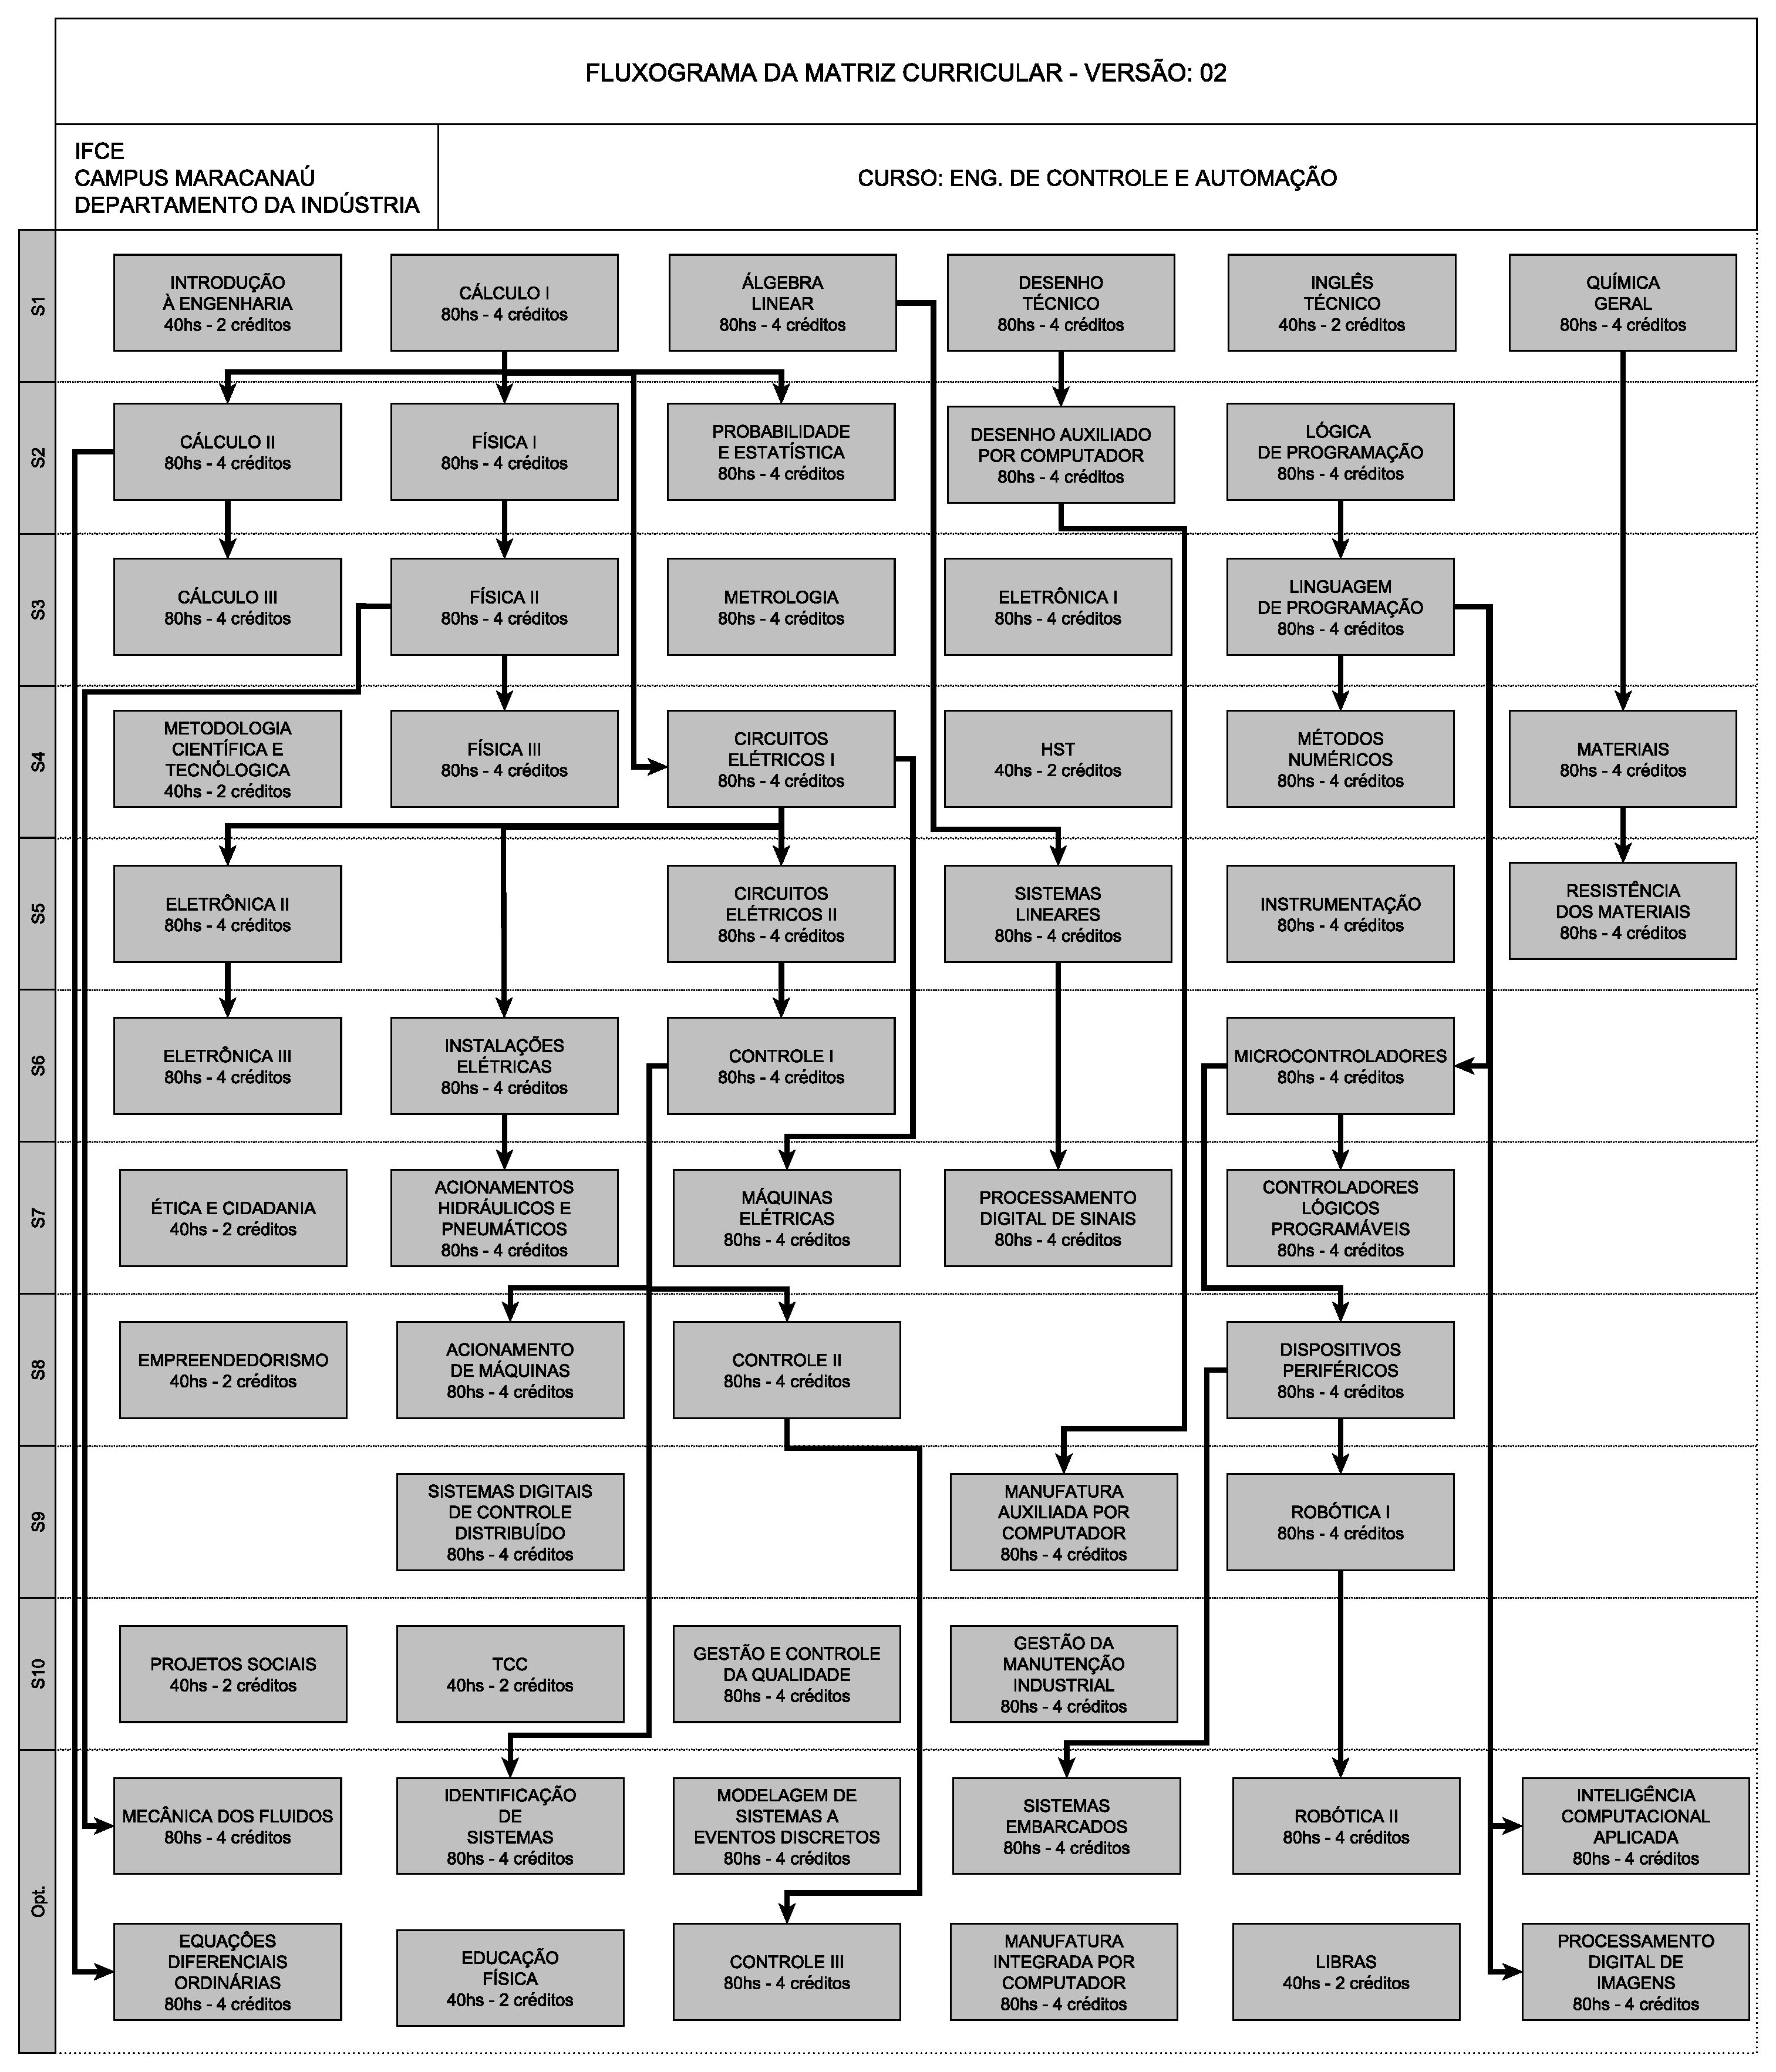
\includepdf[pages={1}]{figuras/CursoECA_Celso.pdf}

\subsection{Estágio Curricular}

O Estágio Curricular Supervisionado constitui componente obrigatório da formação profissional no \NOMECURSO, devendo ser desenvolvido em instituições, empresas ou organizações cuja atuação esteja relacionada à área de formação do estudante. A carga horária mínima exigida para sua integralização é de 160 horas, conforme estabelecido em \citeonline{res259}-Manual de Normalização de Projetos Pedagógicos dos Cursos de Engenharia do IFCE). A conclusão do estágio é condição indispensável para a diplomação.

O Estágio Curricular pode ser iniciado após a conclusão do 5\textsuperscript{o} semestre do curso. Nesse período, o estudante passa a vivenciar experiências reais de trabalho, aplicando fundamentos teóricos adquiridos no ambiente acadêmico, observando processos, rotinas, tecnologias e cultura organizacional. Trata-se de momento formativo em que a prática profissional e a postura ética são diretamente exigidas.

O Estágio Curricular tem como finalidades:

\begin{itemize}
	\item Possibilitar o contato direto com situações reais do ambiente de trabalho;
	\item Favorecer a articulação entre conhecimentos teóricos e práticos;
	\item Contribuir para o desenvolvimento de competências técnicas e comportamentais;
	\item Permitir a compreensão da estrutura e funcionamento do setor produtivo;
	\item Auxiliar na identificação de áreas de maior interesse para futura atuação profissional.
\end{itemize}

O estudante será acompanhado por um professor orientador, responsável pelo acompanhamento sistemático das atividades desenvolvidas. Esse acompanhamento será realizado por meio de reuniões periódicas, presenciais ou remotas, nas quais o discente deverá apresentar registros e relatos das atividades realizadas na organização concedente.

Ao término do estágio, o estudante deverá apresentar um Relatório Final, dentro do prazo estipulado no calendário acadêmico institucional. A avaliação será realizada pelo professor orientador, com base no relatório, na avaliação da organização concedente e na adequação das atividades à área de formação. A conclusão do estágio será registrada mediante os conceitos SATISFATÓRIO ou INSATISFATÓRIO. Caso o resultado seja INSATISFATÓRIO, poderá ser solicitada a reformulação do relatório ou a realização de novo estágio.

Em conformidade com as normativas institucionais expedidas durante os períodos de excepcionalidade (Portaria MEC nº 544/2020 e Ofícios Conjuntos PROEN/PROEXT/PRPI/REITORIA de 2020 e 2021), o Colegiado do Curso autorizou, quando necessário, a realização de atividades de estágio obrigatório e não obrigatório também em formato remoto, conforme registrado em ATA do Colegiado de 05/03/2021 e demais documentos constantes no ANEXO II: Plano de Trabalho Específico – Prática de Estágio Obrigatório/Não Obrigatório.



\subsection{Atividades Complementares}

As Atividades Complementares ou Extra-Curriculares do \NOMECURSO constituem um conjunto de atividades didático-pedagógicas que permitem, no âmbito do currículo, a articulação entre teoria e prática, bem como a complementação das habilidades e saberes necessários a serem desenvolvidos durante o período de formação do profissional.

Tratam-se de atividades diversas, de cunho acadêmico, tecnológico e cultural, que fazem parte da vida escolar do aluno e que são relacionadas com o exercício profissional. De acordo com a \citeonline{cne19}, poderão também ser estimuladas atividades complementares tais como trabalhos de iniciação científica, projetos multidisciplinares, visitas técnicas, trabalhos em equipe, desenvolvimento de protótipos, monitorias, participação em empresas juniores e outras atividades empreendedoras.

As atividades educacionais complementares devem privilegiar a construção de comportamentos sociais e profissionais que as atividades acadêmicas tradicionais, de sala de aula ou de laboratório, não têm condições de propiciar.

Nesta perspectiva, podem ser inseridas as atividades de cunho comunitário e de interesse coletivo, além de privilegiar atividades de monitoria acadêmica e de iniciação científica ou tecnológica que propiciem a participação do estudante na vida da instituição. Podem aqui também serem desenvolvidas atividades esportivas e culturais, além de intercâmbios com instituições estrangeiras.


A carga mínima de atividades complementares não obrigatórias recomendada para o curso abrange um total de \CHCOMP horas-aula. Na sequência são descritas as atividades complementares mais comuns, os critérios para o aproveitamento de carga horária e as exigências para aproveitamento destas atividades complementares. 

Vale destacar que é possível e até incentivada a inclusão e/ou retirada de atividades complementares, como forma do curso se adaptar às novas exigências do mundo do trabalho, sendo que isto será definido pelo NDE e Colegiado do curso.

\subsubsection{Visitas técnicas}

Acontecem a partir do primeiro semestre cursado, com o intuito de facilitar o processo ensino-aprendizagem das
disciplinas cursadas para garantir um bom aproveitamento da mesma.

As visitas técnicas a empresas do Distrito Industrial de Maracanaú e da região metropolitana de Fortaleza são realizadas semestralmente. Uma vez por ano é realizada uma visita técnica a uma empresa de grande porte localizada em regiões fora do estado do Ceará.

\subsubsection{Feiras, Seminários, Congressos e Semanas Tecnológicas}

Os alunos são estimulados a participarem de Seminários, Congressos, Palestras e a participação como Monitor (Auxiliar) em Eventos. Alunos de iniciação científica tem seus trabalhos publicados em Eventos de nível nacional e internacional, participando como apresentadores.

%\subsubsection{Semana de Tecnologias  Industriais (SET-IN)}

O Eixo Tecnológico da Indústria do Campus Maracanaú, com o apoio da direção geral desta unidade e da reitoria do IFCE, realiza a SETIN (Semana de Tecnologias Industriais), que é um evento anual de atividades de pesquisa e extensão. O evento também conta com o apoio de outras instituições e parceiros, tais como o IFCE – Campus Fortaleza, a AEDI (Associação das Empresas dos Distritos Industriais do Estado do Ceará) e o SEBRAE (Serviço Brasileiro de Apoio às Micro e Pequenas Empresas).


\subsubsection{Programa de Monitoria e Bolsas de Trabalho}

A monitoria é uma atividade desenvolvida por alunos de graduação, integrantes de projetos orientados para a diminuição dos índices de evasão e repetência, como também para a melhoria do padrão de qualidade dos cursos de graduação, coordenados por docentes. Além dos monitores bolsistas, remunerados com recursos orçamentários do IFCE, outros alunos podem se integrar aos projetos aprovados, na condição de monitores voluntários.

A Coordenação do \NOMECURSO, juntamente com o Diretoria de Ensino do Campus IFCE / Maracanaú, tem envidado esforços no sentido de fortalecer a componente prática da formação dos nos alunos, futuros engenheiros. Pela própria especificidade do Curso, uma integração eficiente entre a teoria e a prática no processo ensino-aprendizagem é indispensável à formação, com qualidade, dos profissionais exigidos pelo mercado de trabalho. Além disso, as atividades de caráter experimental se constituem, indubitavelmente, em fortes elementos de motivação para os estudantes em nível de Graduação.

O trabalho experimental possibilita o contato e a familiarização com equipamentos, montagens, circuitos, dispositivos e instrumentos de medição. Propicia a comprovação, no laboratório, dos conhecimentos teóricos adquiridos na sala de aula ou por outros meios. Permite ao estudante compreender as limitações e nuances dos modelos teóricos em face da prática de situações reais. Tais aspectos são fundamentais à formação do engenheiro, em particular do \NOMEEGRESSO. A atividade  experimental, instigando o interesse pela investigação científica, também contribui para despertar vocações para a pesquisa.

As disciplinas em que os monitores geralmente atuam constituem a base indispensável ao preparo dos alunos do Curso para o prosseguimento e aprofundamento dos seus estudos no campo da \NOMEENG. Evidencia-se a necessidade de que seja fortalecida a atividade de Monitoria no \NOMECURSO, ao lado de outras iniciativas objetivando incrementar a integração teoria-prática.

No \NOMECURSO, o Programa de Monitoria e de bolsas de trabalho tem os seguintes objetivos principais:

\begin{itemize}
	\item Proporcionar um maior equilíbrio entre teoria e prática no \NOMECURSO, contribuindo para a formação de engenheiros capacitados a enfrentar e resolver problemas colocados pela realidade;
	\item Fortalecer a componente experimental das disciplinas teóricas-práticas, em particular as de formação básica;
	\item Motivar os monitores e demais alunos no estudo das disciplinas - não raro excessivamente teóricas - objetivando a redução dos níveis de evasão no Curso;
	\item Permitir a redução do número de alunos em cada turma de laboratório - viabilizada pela presença de monitores - o que corresponderá a um melhor rendimento, com consequente melhoria da qualidade do ensino ministrado;
	\item Propiciar o surgimento e florescimento de vocações para a docência e a pesquisa, além de promover a cooperação acadêmica entre discentes e docentes.
\end{itemize}

%Atualmente o \NOMECURSO conta com três (3) bolsistas de monitoria e com 20 (vinte) bolsistas de trabalho atuando no apoio às atividades laboratoriais do curso.

\subsubsection{Iniciação Científica com Bolsa ou de Forma Voluntária}

A iniciação científica é a atividade complementar mais importante desenvolvida no curso, onde
o aluno passa a fazer parte de uma equipe de pesquisa, tornando-se responsável pelo
desenvolvimento de um tema. Esse tema se encaixa em um trabalho maior,
envolvendo outros alunos de graduação e de mestrado. O aluno passa a
aprender técnicas não desenvolvidas em sala de aula e passa a se especializar em
determinadas áreas. Além do conhecimento adquirido, existe um grande progresso em
nível individual, quanto à capacidade de trabalho, independência e responsabilidade.

O IFCE oferece Bolsas de Iniciação Científica através dos Programas Institucionais de Bolsas de Iniciação Científica sendo elas do Conselho Nacional de Desenvolvimento Científico e Tecnológico – PIBIC/CNPq, ou da Fundação Cearense de Apoio ao Desenvolvimento Científico e Tecnológico, PIBIC/FUNCAP ambos destinado aos pesquisadores do IFCE com titulação de doutor, para as cotas PIBIC/FUNCAP. As bolsas oferecidas pelo Programa Institucional de Bolsas de Iniciação Científica do Instituto Federal de Educação, Ciência e Tecnologia do Ceará – PIBIC/IFCE são destinadas aos pesquisadores do IFCE com titulação de doutor, mestre ou especialista para as cotas PIBIC/IFCE.

Segundo a conceituação formal do CNPq, ``o PIBIC é um programa centrado na iniciação científica de novos talentos em todas as áreas do conhecimento, administrado diretamente pelas instituições. Voltado para o aluno de graduação e servindo de incentivo à formação, privilegia a participação ativa de bons alunos em projetos de pesquisa com qualidade acadêmica, mérito científico e orientação adequada, individual e continuada. Os projetos culminam com um trabalho final avaliado e valorizado, fornecendo retorno imediato ao bolsista, com vistas à continuidade de sua formação, de modo particular na pós-graduação''.

Além disso, o CNPq menciona que as bolsas de iniciação científica permitem que pesquisadores produtivos engajem estudantes de cursos superiores no processo acadêmico, otimizando a capacidade de orientação à pesquisa na instituição; promovem o aumento da produção científica, com o envolvimento de novos orientadores nas atividades de iniciação à pesquisa científica. Despertam vocação científica e incentivam talentos potenciais entre estudantes de cursos superiores, mediante suas participações em projetos de pesquisa, introduzindo o jovem graduando no domínio do método científico; proporcionam ao bolsista, orientado por pesquisador qualificado, a aprendizagem de técnicas e métodos científicos, bem como estimulam o desenvolvimento do pensar científico e da criatividade, decorrentes das condições criadas pelo confronto direto com os problemas de pesquisa; Despertam no bolsista uma nova mentalidade em relação à pesquisa além de preparar os estudantes para a pós-graduação.

Também são ofertadas bolsas de fomento na Iniciação em Desenvolvimento Tecnológico e Inovação do Conselho Nacional de Desenvolvimento Científico e Tecnológico – PIBITI/CNPq e do Programa Institucional de Bolsas de Iniciação em Desenvolvimento Tecnológico e Inovação do Instituto Federal de Educação, Ciência e Tecnologia do Ceará – PIBITI/IFCE destinados aos pesquisadores do IFCE com titulação de doutor, ou perfil equivalente, e, para as cotas PIBITI/CNPq, pesquisador com titulação de doutor, mestre ou especialista para as cotas PIBITI/IFCE.

As bolsas de Iniciação em Desenvolvimento Tecnológico e Inovação, PIBITI, propiciam à instituição um instrumento de formulação de sua política de inovação tecnológica, através da iniciação tecnológica na graduação, contribuem para a formação e a inserção de estudantes em atividades de pesquisa, desenvolvimento tecnológico e inovação, formação e o engajamento de recursos humanos para atividades de pesquisa, desenvolvimento tecnológico e inovação; contribuem para a formação de recursos humanos que se dedicarão ao fortalecimento da capacidade inovadora das empresas no País, formação do cidadão pleno, com condições de participar de forma criativa e empreendedora na sua comunidade; possibilitam maior interação entre atividades de desenvolvimento tecnológico e inovação, desenvolvidas na graduação e na pós-graduação além de envolver os pesquisadores nas atividades de formação de desenvolvimento tecnológico e inovação.

\subsubsection{Grupos de Pesquisa}

Hoje o \NOMECURSO conta com o Núcleo de Pesquisa Aplicada e Inovação Industrial (NAI)
que contempla os grupos de pesquisa que dão suporte aos alunos no desenvolvimento de pesquisa em nível de iniciação científica. Atualmente são 3 grupos de pesquisa cadastrados no CNPq e certificados pela instituição.

\vspace{0.5cm}

\noindent \textbf{1. Grupo de Inspeção e Análise de Falhas (GIAF)}

Atua no desenvolvimento de pesquisa em inspeção e análise de falhas aplicado ao setor industrial, visando a melhoria contínua dos processos, produtos manufaturados e plantas industriais, de forma a maximizar a vida útil dos equipamentos empregados na indústria. Contribui para a formação de profissionais especializados em inspeção e manutenção. O GIAF conta com a participação de 5 (cinco) pesquisadores e 4 (quatro) estudantes do \NOMECURSO como bolsistas de iniciação científica e 1 (um) estudante como voluntário.

As linhas de pesquisa do GIAF são:
\begin{itemize}
	\item Análise Microestrutural de Metais
	\item Corrosão
	\item Inspeção e Ensaios em Materiais
	\item Manutenção Preventiva e Preditiva
\end{itemize}

\noindent \textbf{2. Grupo de Pesquisa em Sistemas Inteligentes (GPSI)}

Atua no desenvolvimento de inovações científicas e tecnológicas aplicadas às áreas de Automação Industrial, Energia e Manutenção Industrial. Contribui para a melhoria contínua dos processos, plantas industriais e para a formação de profissionais especializados, atendendo às necessidades regionais e ao crescimento do parque industrial. O GPSI conta com a participação de 11 (onze) pesquisadores e 4 (quatro) estudantes do \NOMECURSO como bolsistas de iniciação científica e 1 (um) estudante como voluntário.

As linhas de pesquisa do GPSI são:
\begin{itemize}
	\item Aproveitamento de Energias Alternativas e Eficiência Energética
	\item Controle e Automação Aplicados a Processos de Fabricação
	\item Inspeção e Manutenção Preditiva
\end{itemize}


\noindent \textbf{3. Grupo de Pesquisa Energias Renováveis (GPER)}

Atua no desenvolvimento de inovações científicas e tecnológicas aplicadas às áreas de Automação Industrial, Energia, Manutenção Industrial. Contribui para a melhoria contínua dos processos de geração de energia, atuando no desenvolvimento tecnológico e sustentável do parque industrial, visando diminuir os impactos da crise de energia e meio ambiente, além de contribuir para a formação de profissionais especializados, atendendo às necessidades regionais. O GPER conta com a participação de 11 (onze) pesquisadores e 4 (quatro) estudantes do \NOMECURSO como bolsistas de iniciação científica e 1 (um) estudante como voluntário.

As linhas de pesquisa do GPER são:
\begin{itemize}
	\item Controle e Processamento de Energia
	\item Mecânica Aplicada à conservação do meio ambiente
	\item Energia Eólica
	\item Energia fotovoltáica
\end{itemize}

\subsubsection{Bolsa de Monitoria e de Trabalho}

O \NOMECURSO dispõe através de programas de auxílio ao discente, bolsistas para atividades de monitoria e de trabalho atuando no apoio às atividades laboratoriais do curso. A atividade de monitoria é desenvolvida dentro de uma disciplina, por um aluno que já a tenha cursado e que tenha conseguido uma nota mínima de 7,0. Nesta atividade, há o contato com colegas mais novos, desenvolvendo no aluno monitor aspectos mais abrangentes de caráter didático-pedagógico, bem como a necessidade de aprofundamento na disciplina em questão.

\subsubsection{Estágios não Obrigatórios}
Estágios de curta duração também estão disponíveis para o aluno de graduação.
Nesses estágios diferentes empresas e diferentes processos produtivos podem ser
conhecidos, dando um maior embasamento e maior conhecimento no campo de
trabalho futuro do aluno.


%\subsubsection{Viagens de Estudo}
%Atividades como viagens de estudo já são usados no presente momento como elementos motivadores e %instrumentos pedagógicos complementares do curso de graduação. As visitas ocorrem aos parques industriais %do estado do Ceará. A programação é feita dentro do contexto de cada disciplina, havendo o acompanhamento %do professor responsável.

\subsubsection{AeroDesign}

O IFCE, Campus Maracanaú, conta com uma equipe de projeto de aeromodelos, a AirLamp Aerodesign - IFCE. Esta é formada, atualmente, por alunos dos cursos de Engenharia Mecânica e Engenharia de Controle e Automação do campus. A AirLamp visa tirar a Engenharia do papel projetando aeromodelos eficientes, com o menor custo possível, materiais inovadores a fim de competir na competição organizada pela SAE Brasil. A inexistência de um prérequisito tem como objetivo a participação de alunos de diversos níveis, incentivando o trabalho em equipes e uma maior adaptação do aluno ao ambiente do curso.

\subsubsection{Enactus}

A Enactus trata-se de uma organização internacional que mobiliza estudantes, acadêmicos e líderes de negócios que estão comprometidos a usar o poder da ação empreendedora para possibilitar o progresso no mundo. Guiados por professores conselheiros e especialistas em negócios, os estudantes
participantes formam times em seus campi para criar e implementar projetos comunitários que empoderam pessoas para melhorar sua qualidade e padrão de vida. Essa experiência não somente transforma vidas, mas também ajuda os estudantes a desenvolverem o tipo de talento e perspectiva necessários para tornarem-se líderes eficazes e direcionados ao valor.

Uma série anual de campeonatos regionais e nacionais fornece um fórum para que os times possam apresentar os resultados dos seus projetos, e para que sejam avaliados por líderes de negócios, que atuam como juízes. Os campeões nacionais de cada país avançam para a prestigiada Enactus World Cup. Além do aspecto comunitário do programa, oportunidades significativas são criadas para o aprendizado e trocas de experiências entre gerações, além de expor estudantes e ex-alunos às empresas que procuram um novo talento.

O Time Enactus IFCE Maracanaú tem como objetivo ajudar comunidades do entorno do campus em seu desenvolvimento. A nível de instituição, a participação no time é considerada uma atividade de extensão. A inexistência de um prérequisito tem como objetivo a participação de alunos de diversos níveis, incentivando o trabalho em equipes e uma maior adaptação do aluno ao ambiente do campus.


%\subsubsection{Empresa Júnior}
%A empresa júnior de engenharia mecânica – atualmente denominada I9 Consultoria –
%foi criada em 1995 e tem a finalidade de desenvolver as vocações empresariais dos
%estudantes do curso. A empresa atua diretamente no mercado como consultora e
%executora de projetos. O suporte é dado pelos professores e pelos laboratórios do
%EMC, sempre que houver necessidade. Trata-se também de uma atividade integradora,
%onde os estudantes são treinados para o dia a dia de trabalho em suas atividades
%futuras de engenheiros-empreendedores.

%\subsubsection{Programa Especial de Treinamento – PET}
%O Grupo PET Metrologia e Automação da UFSC, foi fundado em 1980 e conta com a
%participação de estudantes de Engª Mecânica. Inclui a organização e a participação
%seminários, palestras e cursos com o intuito de aproximar os estudantes ao mercado
%de trabalho. Tem também como meta a realização de projetos técnico-científicos de
%engenharia, em parceria com pequenas, médias e grandes empresas do setor metalmecânico
%brasileiro.


\subsubsection{Cooperação Internacional}

O Programa de Bolsas IFCE Internacional visa consolidar a internacionalização do IFCE, propiciando a interiorização destas ações, bem como possibilitar a participação de alunos de diferentes níveis de ensino, oportunizando a participação de discentes do ensino técnico cuja oferta para mobilidade internacional é quase inexistente.
A fim de intensificar as atividades já desenvolvidas com instituições de ensino estrangeiras parceiras do IFCE, os discentes selecionados pelo presente programa através de edital serão enviados para cursar um semestre acadêmico em instituições de ensino de excelência em diferentes países.
Além destas parcerias já consolidadas, outras instituições e indústrias têm sido utilizadas pelos alunos, colocando-se atualmente, como uma necessidade para a formação, tanto pelo aprendizado de novas línguas, quanto pelo contato com outras culturas.

\subsubsection{Outras Atividades Complementares}
Tratam-se de outras atividades complementares também aceitas no curso:
\begin{itemize}
	\item Assistir a palestras
	\item Participação como debatedor em eventos na área do curso
	\item Apresentação de trabalhos como expositor em eventos na área
	\item Participação em projetos e programas de extensão promovidos ou não pelo IFCE
	\item Participação em cursos de extensão na área do curso de graduação ministrados ou não pelo IFCE
	\item Participação em cursos de extensão em geral
	\item Participação em atividades ou eventos culturais organizados pelo IFCE ou por outras instituições de Ensino Superior
	\item Participação em atividades nos centros acadêmicos ou diretórios de estudantes
	\item Participação em órgãos de direção de entidade de natureza acadêmica
	\item Representação em colegiados acadêmicos ou administrativos do IFCE
	\item Aprovação em disciplinas conexas
	\item Cursos de ensino a distância em áreas afins ao curso
	\item Outras atividades relativas a quaisquer colaborações em situações acadêmicas
\end{itemize}

Desta-se novamente que é possível e até incentivada ainclusão e/ou retirada de atividades complementares, como forma do curso se adaptar às novasexigências do mundo do trabalho, sendo que isto será definido pelo NDE e Colegiado do curso.

\subsubsection{Carga Horária por Modalidade de Atividade Complementar}

O aproveitamento da carga horária seguirá os critérios estabelecidos na Tab. \ref{tab12} Deverá ser respeitado o limite de carga horária por cada Atividade Complementar descrita. A carga horária que exceder o cômputo geral, de acordo com as modalidades, não será aproveitada.

\begin{longtable}{|p{8.5cm}|p{3.5cm}|p{2cm}|}
	
	\caption{Carga horária por modalidade de atividade complementar}\label{tab12} 
	
	\vspace{-0.25cm}
	
	%\multicolumn{3}{c}{\textbf{Tabela 6. Carga horária por modalidade de atividade complementar}} 
	
	\\ \hline 
	
	\cellcolor{\cinza}Atividade & \cellcolor{\cinza}CH por Atividade & \cellcolor{\cinza}CH Total \\ 
	
	\hline
	
	Visita técnica & Até 4h por visita & Até 60h \\ 
	
	\hline 
	
	Feiras, Seminários, Congressos e Semanas Tecnológicas & Até 20h por evento & Até 60h \\
	
	\hline
	
	Programa de Monitoria e Bolsas de Trabalho & Até 30h por semestre & Até 60h \\
	
	\hline
	
	Iniciação Científica com Bolsa ou de Forma Voluntária & Até 20h por pesquisa & Até 80h \\
	
	\hline
	
	Grupos de Pesquisa & Até 20h por pesquisa & Até 80h \\
	
	\hline
	
	Bolsa de Monitoria e de Trabalho & Até 30h por semestre & Até 60h \\
	
	\hline
	
	Estágios não Obrigatórios & Até 70h & Até 70h \\
	
	\hline
	
	AeroDesign & Até 30h por semestre & Até 60h \\ 
	
	\hline
	
	Enactus & Até 30h por semestre & Até 60h \\
	
	\hline
	
	Cooperação Internacional & Até 40h por disciplina & Até 200h\\
	
	\hline
	
	Assistir a palestras & Até 4h por evento & Até 60h \\
	
	\hline
	
	Participação como debatedor em eventos na área do curso & Até 8h por evento & Até 60h \\
	
	\hline
	
	Apresentação de trabalhos como expositor em eventos na área & Até 20h por trabalho & Até 60h \\
	
	\hline
	
	Participação em projetos e programas de extensão promovidos ou não pelo IFCE & Até 20h por atividade & Até 80h \\
	
	\hline
	
	Participação em cursos de extensão na área do curso de graduação ministrados ou não pelo IFCE & Até 30h por curso & Até 60h \\
	
	\hline
	
	Participação em cursos de extensão em geral & Até 5h por curso & Até 20h \\
	
	\hline
	
	Participação em atividades ou eventos culturais organizados pelo IFCE ou por outras instituições de Ensino Superior & Até 10h por atividade & Até 40h \\
	
	\hline
	
	Participação em atividades nos centros acadêmicos ou diretórios de estudantes & Até 4h por atividade & Até 30h \\
	
	\hline
	
	Participação em órgãos de direção de entidade de natureza acadêmica & Até 10h por semestre & Até 40h \\
	
	\hline
	
	Representação em colegiados acadêmicos ou administrativos do IFCE & Até 10h por semestre & Até 40h \\
	
	\hline
	
	Aprovação em disciplinas conexas & Até 40h por disciplina & Até 80h \\
	
	\hline
	
	Cursos de ensino a distância em áreas afins ao curso & Até 60h & Até 60h \\
	
	\hline
	
	Outras atividades relativas a quaisquer colaborações em situações acadêmicas & Até 40h & Até 40h \\
	
	\hline
	
\end{longtable} 

\subsubsection{Aproveitamento de Atividades Complementares}

Ficam estabelecidas as seguintes exigências para o aproveitamento das Atividades Complementares, conforme Tab. \ref{tab13}. O controle do cumprimento dos créditos referentes às Atividades Complementares é de responsabilidade do coordenador do curso, a quem cabe avaliar a documentação exigida para a validação da atividade.

\begin{longtable}{|p{8.5cm}|p{5.5cm}|}
	
	\caption{Aproveitamento de atividades complementares}\label{tab13}
	
	\vspace{-0.25cm}
	
	%\multicolumn{2}{c}{\textbf{Tabela 7. Exigências para aproveitamento de atividades complementares}} 
	
	\\ \hline 
	
	\cellcolor{\cinza}Atividade & \cellcolor{\cinza}Documentação Necessária \\ 
	
	\hline
	
	Visita técnica & Declaração emitida pelo professor responsável atestando a quantidade de horas e que a mesma não foi registrada em diário como atividade de alguma disciplina \\ 
	
	\hline 
	
	Feiras, Seminários, Congressos e Semanas Tecnológicas & Certificado de presença \\
	
	\hline
	
	Programa de Monitoria e Bolsas de Trabalho & Relatório do professor orientador \\
	
	\hline
	
	Iniciação Científica com Bolsa ou de Forma Voluntária & Relatório do professor orientador \\
	
	\hline
	
	Grupos de Pesquisa & Relatório do professor orientador \\
	
	\hline
	
	Bolsa de Monitoria e de Trabalho & Relatório do professor orientador \\
	
	\hline
	
	Estágios não Obrigatórios & Declaração emitida pelo setor de estágios \\
	
	\hline
	
	AeroDesign & Declaração de participação emitida pelos líderes da equipe \\ 
	
	\hline
	
	Enactus & Declaração de participação emitida pelos líderes do time \\
	
	\hline
	
	Cooperação Internacional & Declaração emitida pelo setor responsável \\
	
	\hline
	
	Assistir a palestras & Atestado de participação \\
	
	\hline
	
	Participação como debatedor em eventos na área do curso & Atestado de participação \\
	
	\hline
	
	Apresentação de trabalhos como expositor em eventos na área & Atestado de participação \\
	
	\hline
	
	Participação em projetos e programas de extensão promovidos ou não pelo IFCE & Declaração emitida pelo professor responsável atestando a quantidadede horas e que a mesma não foi registrada em diário como atividade de alguma disciplina \\
	
	\hline
	
	Participação em cursos de extensão na área do curso de graduação ministrados ou não pelo IFCE & Atestado de participação \\
	
	\hline
	
	Participação em cursos de extensão em geral & Atestado de participação \\
	
	\hline
	
	Participação em atividades ou eventos culturais organizados pelo IFCE ou por outras instituições de Ensino Superior & Atestado de participação \\
	
	\hline
	
	Participação em atividades nos centros acadêmicos ou diretórios de estudantes & Atas de reunião e relatório de atividades \\
	
	\hline
	
	Participação em órgãos de direção de entidade de natureza acadêmica & Atas de reunião e relatório de atividades \\
	
	\hline
	
	Representação em colegiados acadêmicos ou administrativos do IFCE & Atas de reunião e relatório de atividades \\
	
	\hline
	
	Aprovação em disciplinas conexas & Histórico constando a nota obtida e o programa da disciplina\\
	
	\hline
	
	Cursos de ensino a distância em áreas afins ao curso & Certificado de conclusão\\
	
	\hline
	
	Outras atividades relativas a quaisquer colaborações em situações acadêmicas & Certificado de realização\\
	
	\hline
	
\end{longtable} 

Ao longo do semestre letivo, o aluno deverá apresentar os comprovantes cabíveis e suas respectivas cópias ao coordenador do curso, que os apreciará, podendo recusar a atividade se considerar insatisfatória e/ou o desempenho do aluno. Sendo aceita a atividade realizada pelo aluno, cabe ao coordenador do curso atribuir a carga horária correspondente.

%Quando da apresentação dos comprovantes, o coordenador deverá atestar as cópias, mediante o documento original e arquivá-las na pasta de Atividades Complementares do aluno.

É vedado o cômputo concomitante ou sucessivo, como Atividade Complementar, de cargas horárias ou conteúdos, trabalhos, atividades ou práticas próprias das disciplinas do currículo pleno, ou destinado à elaboração e defesa do PFC, ou desenvolvidos nos estágios curriculares.

De atos ou decisões do coordenador do curso caberá recurso à Direção de Ensino do campus.

\subsection{Trabalho de Conclusão de Curso (PFC)}

O PFC trata-se de um trabalho acadêmico de caráter obrigatório que tem o objetivo de promover a consolidação dos conhecimentos adquiridos no decorrer do curso. Além disso, visa a iniciação e envolvimento do aluno de graduação no campo da pesquisa científica.

Quando da elaboração do trabalho para apresentação, o aluno deve se matricular na disciplina de PFC, sendo que, para tal, é obrigatório que este tenha cumprido no minimo de 80\% dos crétidos obrigatórios constantes na matriz do curso.  
A entrega de um pré-projeto de PFC constitui pré-requisito obrigatório para que possa matricular-se na disciplina. 

Desta feita, o professor da disciplina de PFC, além de cumprir o programa constante no respectivo PUD, atuará como um coordenador do trabalho implementado pelo aluno e seu professor orientador.

O aluno pode optar por apresentar um artigo que tenha sido aceito para publicação em periódico ou artigo que tenha sido apresentado em um evento científico, desde que conste o nome do \textbf{professor orientador} na lista de autores. O artigo será submetido à análise do professor de PFC que emitirá um parecer quanto à relevância e atualidade do trabalho. Caso o artigo seja aceito \textbf{sem alterações} como substituto da monografia, o aluno poderá passar para a fase de apresentação pública do trabalho. Caso contrário, o aluno deverá iniciar o desenvolvimento de uma monografia (baseada no Manual de Normalização de Trabalhos Acadêmicos do IFCE, aprovado através da Resolução 034/Consup, de 27 de março de 2017 e disponível no endereço \web{https://ifce.edu.br/proen/bibliotecas/normalizacao-de-trabalhos-academicos}) ou artigo (científico ou técnico) visando a publicação em periódico de circulação nacional ou internacional com avaliação Qualis A ou B nas áreas de engenharia, computação ou interdisciplinar da CAPES.

O desenvolvimento do trabalho será acompanhado por um professor orientador que proporciona aos alunos subsídios para construir algo, tais como: definição do tema, acompanhamento das atividades práticas e/ou teóricas, revisão da parte escrita e conclusão do trabalho. A disciplina de PFC terá um professor responsável que atuará como coordenador das atividades implementadas pelo aluno e seu professor orientador, o qual acompanhará o cumprimento das seguintes etapas:

\begin{itemize}
	\item Entrega do Pré-Projeto do PFC ou artigo publicado;
	\item Entrega do termo de aceite de orientação assinado pelo professor orientador;
	\item Entrega de relatórios da execução de atividades referentes à monografia ou artigo;
	\item Entrega da versão impressa para apresentação pública;
	\item Apresentação pública da monografia ou artigo;
	\item Entrega da versão final da monografia ou artigo.
\end{itemize}

Os prazos de cada uma das etapas acima serão definidos pelo professor da disciplina de PFC juntamente com a coordenação
do \NOMECURSO. Somente após a conclusão da última etapa pelo aluno será lançada a nota da disciplina no sistema acadêmico.

\subsubsection{Entrega do Pré-Projeto do PFC}

O Pré-Projeto é um documento que apresenta a percepção do aluno quanto ao trabalho que será executado. Este documento é importante para orientar as atividades e permitir um bom planejamento do aluno. A viabilidade do projeto será analisada pelo orientador e pelo professor da disciplina de PFC, o qual poderá sugerir ajustes com o objetivo de melhorar as chances de conclusão no tempo previsto.

O Pré-Projeto deve ser apresentado à coordenação de curso como pré-requisito para matrícula na disciplina de PFC. A estrutura mínima do documento contemplar:

\begin{itemize}
	\item Capa;
	\item Tema;
	\item Problema;
	\item Objetivos;
	\item Justificativa;
	\item Metodologia;
	\item Cronograma;
	\item Referências Bibliográficas.
\end{itemize}

\subsubsection{Entrega do termo de aceite de orientação assinado pelo professor orientador}

O termo é um compromisso assumido pelo professor orientador e seu respectivo orientando com relação ao cumprimento das
etapas e do cronograma de elaboração e entrega do PFC. É importante ressaltar que o professor orientador é responsável
pela qualidade e garantia de aprovação do PFC. O termo deverá obedecer ao modelo descrito a seguir.

\begin{verbatim}
	TERMO DE ACEITE DE PFC
	
	Eu, <nome do professor>, professor do Instituto Federal de Educação,
	Ciência e Tecnologia de Ceará – Campus Maracanaú, Eixo Tecnológico da Indústria,
	declaro para os devidos fins, que aceito orientar o(a) aluno(a) <nome completo
	do(a) aluno(a)> do <nome do curso> na execução do Trabalho de Conclusão de Curso
	cujo título é <título do trabalho>.
	
	Maracanaú – CE, dia / mês / ano
	
	----------------------------------
	assinatura do professor orientador
	
\end{verbatim}

\subsubsection{Entrega de relatórios da execução de atividades referentes ao PFC}

Os relatórios têm o objetivo de auxiliar o acompanhamento das atividades previstas para a elaboração do PFC. O
professor da disciplina de PFC poderá solicitar ao aluno e/ou ao professor orientador que façam ajustes necessários à
boa qualidade do trabalho.

\subsubsection{Entrega da versão para apresentação pública}

De forma a atender as demandas do professor da disciplina de PFC e da respectiva banca examinadora, devem ser entregues a versão digital (em pdf) do texto para apresentação, bem como cópias impressas com encadernação simples (caso necessárias) ao professor da disciplina de PFC, que terá a responsabilidade de repassar essas a cada membro da banca examinadora.

\subsubsection{Apresentação pública do PFC}

Trata-se de uma seção pública tendo uma banca examinadora composta pelo professor orientador, como presidente, e mais dois membros, sendo pelo menos um deles do Instituto Federal de Educação, Ciência e Tecnologia do Ceará. Um dos membros da banca, à exceção do presidente, pode ser de uma empresa industrial ou de outra instituição, pública ou privada, de ensino superior de graduação em áreas tecnológicas.  Todos os membros da banca devem possuir, pelo menos, pós-graduação em nível de especialização.  A apresentação do PFC é pública, portanto aberta para qualquer membro da sociedade que desejar assistir.

A apresentação é dividida em quatro etapas:

\begin{itemize}
	\item Apresentação do trabalho pelo proponente: utiliza recursos multimídia para melhor visualização dos membros da banca e de todas as pessoas que estiverem presentes. O tempo de duração da apresentação deve ser de no máximo 30 (trinta) minutos.
	\item Arguições e considerações por parte da banca: após a apresentação do trabalho, cada membro da banca inicia o processo de arguição e considerações, onde são apontadas sugestões para melhoria do trabalho e possíveis correções. Após todos os membros da banca concluírem suas arguições e considerações, o presidente pode determinar um tempo para questionamentos e considerações das pessoas que estão assistindo a defesa.
	\item Reunião da banca com o professor da disciplina de PFC: é a última etapa da apresentação e ocorre para que os membros da banca e o professor da disciplina de PFC discutam, de maneira reservada, as características do trabalho apresentado e deliberem pela nota do trabalho.
	\item Composição da nota da disciplina de PFC: cada membro da banca juntamente com o professor da disciplina de PFC atribuirão uma nota de 0 (zero) a 10 (dez), em formulário específico, e a média aritmética dessas notas será a nota final da disciplina de PFC. Essa etapa dará origem ao Parecer de Trabalho de Conclusão de Curso, que será o documento oficial a ser considerado para registro da nota final atribuída à disciplina de PFC.
	\item Comprovação de participação dos membros da banca: cada membro da banca examinadora receberá uma declaração, pela Coordenação do \NOMECURSO, que comprovará a respectiva participação de cada um deles na defesa do PFC junto ao Instituto Federal de Educação, Ciência e Tecnologia do Ceará e a qualquer outra instituição de natureza pública ou privada.
\end{itemize}

\subsubsection{Entrega da versão final do PFC}

Após a apresentação do PFC, o(a) aluno(a) deve efetuar as correções e/ou melhorias propostas pela banca examinadora. A aceitação da versão final com suas respectivas correções e/ou melhorias será confirmada por meio de um consenso entre o professor orientador e o professor da disciplina de PFC.

A validade das notas atribuídas ao trabalho apresentado está condicionada à entrega %de 01 (uma) cópia impressa da versão final, encadernada em capa dura com letras douradas, assim como a entrega  
do arquivo eletrônico em mídia digital, o qual será disponibilizado para acesso público no Sistema de Bibliotecas do IFCE - SIBI (no endereço eletrônico \web{http://biblioteca.ifce.edu.br/}). É importante ressaltar que nesta versão final deve conter a ficha catalográfica, fornecida pela biblioteca do \textit{campus}, e o Parecer de Trabalho de Conclusão de Curso, fornecido pela coordenação do \NOMECURSO.

A nota da disciplina de PFC será distribuída igualmente na média dos 02 (dois) períodos, N1 e N2, do semestre letivo.




